%
% LaTeX report template 
%

% This is a comment: in LaTeX everything that in a line comes
% after a "%" symbol is treated as comment

\documentclass[11pt, a4paper]{article}
\usepackage{graphicx}
\usepackage{amsmath}
\usepackage{listings}


\title{Assignment No 5} % Title

\author{Prasanna Bartakke EE19B106} % Author name

\date{\today} % Date for the report
\begin{document}		
		
\maketitle % Insert the title, author and date
\section{Introduction}
%Create new section;it is autonumbered
We wish to solve for the currents in a resistor. The currents depend on the shape of the resistor and we also want to know which part of the resistor is likely to get hottest.

\section{Equations}
A cylindrical wire is soldered to the middle of a copper plate and its voltage is held at 1 Volt. One side of the plate is grounded, while the remaining are floating. The plate is 1 cm by 1 cm in size.\\
Conductivity
\begin{equation}
\vec{j} = \sigma\vec{E}
\end{equation}
Electric field is the gradient of the potential
\begin{equation}
\vec{E} = -\nabla\phi
\end{equation}
Continuity of charge
\begin{equation}
\nabla\vec{j} = -\frac{\partial \rho}{\partial t}
\end{equation}
Combining the equations ans substituting $\rho$ = 0, we get
\begin{equation}
\nabla^2 \phi = 0
\end{equation}
\section{Defining parameters and Initialising potential}
We choose a 25x25 grid with a circle of radius 8 centrally located maintained at V = 1V by default. We also choose to run the difference equation for 1500 iterations by default.
We start by creating an zero 2-D array of size Nx x Ny. then a list of coordinates
lying within the radius is generated and these points are initialized to 1.
   \begin{figure}[!tbh]
   	\centering
   	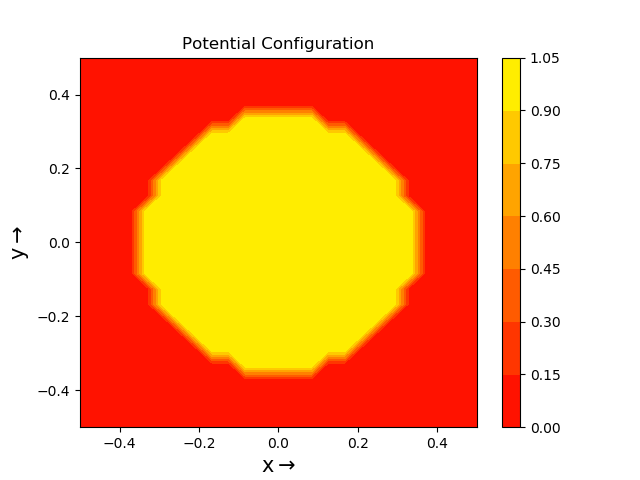
\includegraphics[scale=0.5]{fig0.png}  % Mention the image name within the curly braces. Image should be in the same folder as the tex file. 
   	\caption{Initial Potential}
   	\label{fig:sample}
   \end{figure} 
\section{Performing iterations}
	\subsection{Updating the potential}
	We convert the differential equation(4) to the following difference equation.
	\begin{equation}
	\phi_{i, j} = \frac{\phi_{i-1, j} + \phi_{i, j-1} + \phi_{i+1, j} + \phi_{i, j+1}}{4}
	\end{equation}
	\begin{verbatim}
	def update_phi(phi,phiold):
    phi[1:-1,1:-1]=0.25*(phiold[1:-1,0:-2]+ phiold[1:-1,2:]+ phiold[0:-2,1:-1] + phiold[2:,1:-1])
    return phi
	\end{verbatim}
 	\subsection{Enforcing Boundary Conditions}
	The bottom boundary is grounded. The other 3 boundaries have a normal potential difference zero.
	\begin{verbatim}
	def boundary(phi,mask = np.where(X**2+Y**2<(0.35)**2)):
    #Left
    phi[:,0]=phi[:,1]
    #Right
    phi[:,Nx-1]=phi[:,Nx-2] 
    #Top 
    phi[0,:]=phi[1,:] 
    #Bottom
    phi[Ny-1,:]=0
    #wire
    phi[mask]=1.0
    return phi
	\end{verbatim}
	\subsection{Calculating error after each iteration}
	\begin{verbatim}
	err = np.zeros(Niter)
for k in range(Niter):
    phiold = phi.copy()
    phi = update_phi(phi,phiold)
    phi = boundary(phi)
    err[k] = np.max(np.abs(phi-phiold))
	\end{verbatim}
	\subsection{Plotting Error}
	Plot the errors on semi-log and log-log plots. As we can see that the error
falls slowly and this is one of the reasons why this method of solving the
Laplace equation is not preferred.
\begin{figure}[!tbh]
   	\centering
   	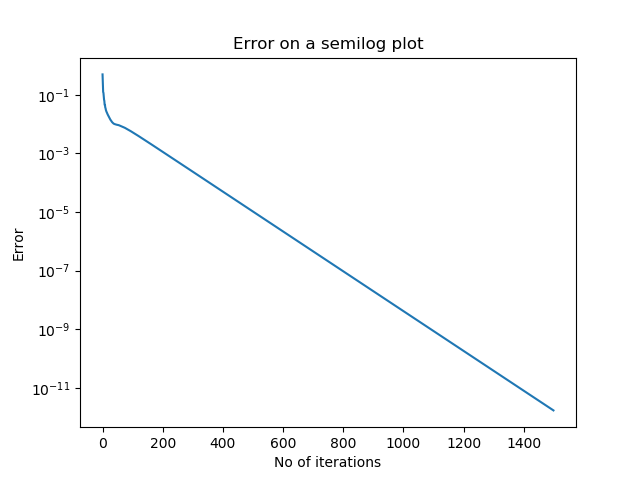
\includegraphics[scale=0.5]{fig1.png}  % Mention the image name within the curly braces. Image should be in the same folder as the tex file. 
   	\caption{Semilog plot of errors}
   	\label{fig:sample}
   \end{figure} 
   
   \begin{figure}[!tbh]
   	\centering
   	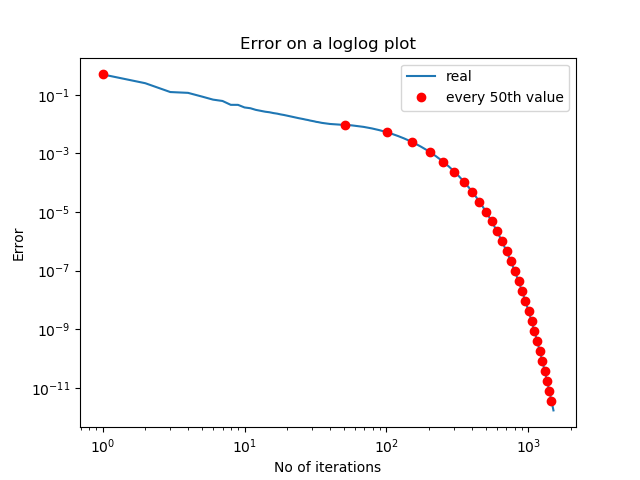
\includegraphics[scale=0.5]{fig2.png}  % Mention the image name within the curly braces. Image should be in the same folder as the tex file. 
   	\caption{Loglog plot of errors}
   	\label{fig:sample}
   \end{figure} 
   
 
\section{Fitting the error}
The error is a decaying potential for higher iterations. We attempt to fit a function 
\begin{equation}
y = Ae^{Bx}
\end{equation}
\begin{equation}
log(y) = log(A) + Bx
\end{equation}
We estimate log(A) and B with the least squares method.
fit1 is considering all the iterations and fit2 is considering iterations from 500 onwards.
\begin{figure}[!tbh]
   	\centering
   	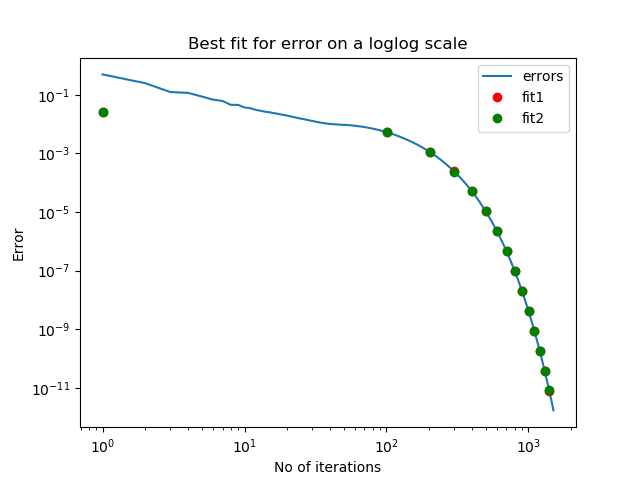
\includegraphics[scale=0.5]{fig3.png}  % Mention the image name within the curly braces. Image should be in the same folder as the tex file. 
   	\caption{Best fit of errors}
   	\label{fig:sample}
   \end{figure} 
   There is very little difference between the two fits.
   
\section{Plotting maximum error}
\begin{figure}[!tbh]
   	\centering
   	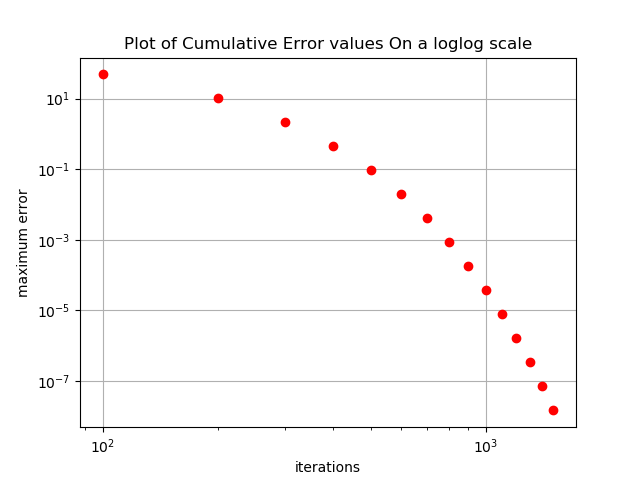
\includegraphics[scale=0.5]{fig5.png}  % Mention the image name within the curly braces. Image should be in the same folder as the tex file. 
   	\caption{Cumulative error values on a log log scale}
   	\label{fig:sample}
   \end{figure} 
   

\section{Plotting Potential}
\begin{figure}[!tbh]
   	\centering
   	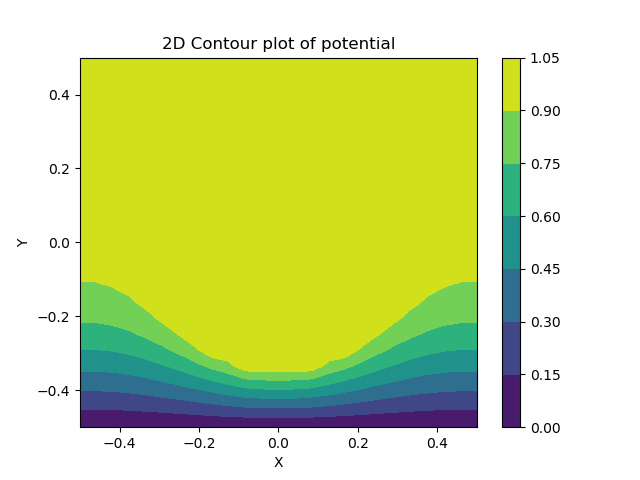
\includegraphics[scale=0.5]{fig6.png}  % Mention the image name within the curly braces. Image should be in the same folder as the tex file. 
   	\caption{2d plot of potential}
   	\label{fig:sample}
   \end{figure} 
\begin{figure}[!tbh]
   	\centering
   	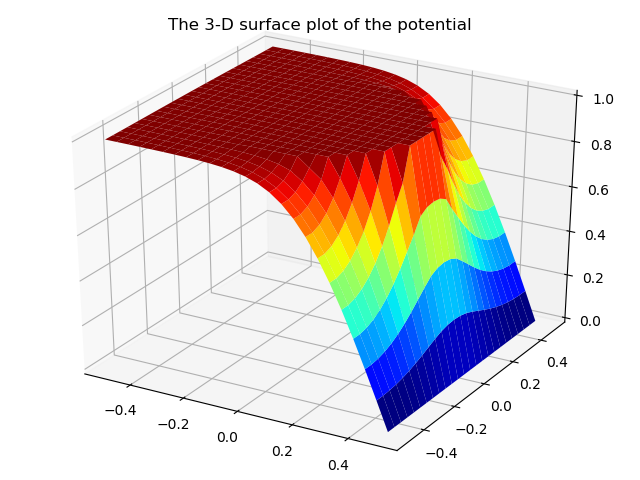
\includegraphics[scale=0.5]{fig7.png}  % Mention the image name within the curly braces. Image should be in the same folder as the tex file. 
   	\caption{3d plot of potential}
   	\label{fig:sample}
   \end{figure}
   
\section{Calculating current density}
\begin{equation}
J_{x, ij} = \frac{\phi_{i, j-1} - \phi{i, j+1}} {2}
\end{equation}
\begin{equation}
J_{y, ij} = \frac{\phi_{i-1, j} - \phi{i+1, j}} {2}
\end{equation}
\begin{figure}[!tbh]
   	\centering
   	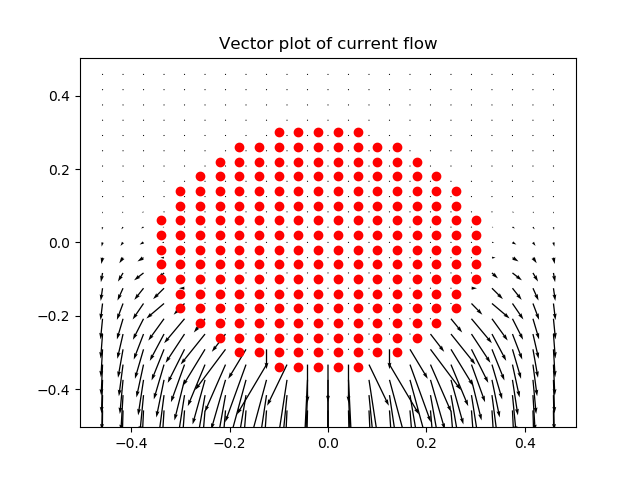
\includegraphics[scale=0.5]{fig8.png}  % Mention the image name within the curly braces. Image should be in the same folder as the tex file. 
   	\caption{Vector plot of current}
   	\label{fig:sample}
   \end{figure}
From the current density plot, we can see that hardly any current flows through the top part of  the wire. We can conclude that the lower surface being grounded, the easiest way for charge carriers to flow from the electrode would be directly through the lower half of the wire, thus
avoiding a longer, more resistive path through the top half of the wire.

\section{Conclusion}
We can find solution to Laplace's equation for a given system using a finite differentiation approximation. The error is seen to decay at a gradual pace. Thus the chosen method of solving Laplace’s equation is inefficient. 
On analysing the vector plot of the currents, we can conclude that the current was mostly restricted to the bottom of the wire.
\end{document}



 